\documentclass{article}
\usepackage[margin=1in]{geometry}
\usepackage{amsmath,amsfonts,amsthm}
\usepackage{graphicx}
\graphicspath{.}

\begin{document}

\section{Appeal}

The grader suggests that I did not fully solve the problem because I did not connect my final claim to the equations I gave at the beginning of my proof.

The only details which I did not explicitly include are the idea that, if $(x,y,z)$ denote the cartesian coordinates of $P$, you can express $OH^2 = x^2+y^2$ and $HP = z$.
However, these are intrinsic features in the 3-d cartesian coordinate system and its metric, which are both assumed in the initial construction of the problem.
The substitution of $x$, $y$, and $z$ are also standard conventions in the cartesian coordinate system.

Once these substitutions are made, our original equation is equivalent to our final claim.
$$HP^2 = \frac{1-OH^2}{2} \implies z^2 = \frac{1-x^2-y^2}{2}$$

\section{Response}

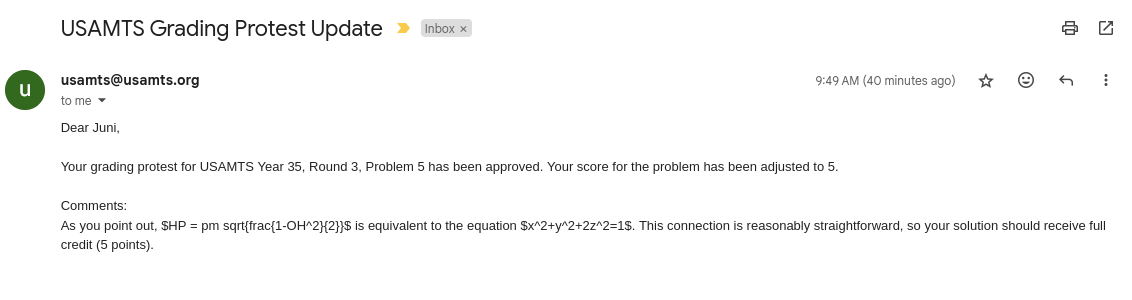
\includegraphics[width=\textwidth]{round3/p5_appeal_response.png}
\end{document}